\section{Ejercicio 1}

\subsection{Enunciado}
Programar un tipo de tarea \textbf{TaskConsola}, que simulará una tarea interactiva.
La tarea debe realizar \textit{n} llamadas bloqueantes, cada una de una duración al azar entre \textit{bmin} y \textit{bmax} (inclusive). 
Luego ejecutará 1 tic cada vez. 
La tarea debe recibir tres parámetros: \textit{n}, \textit{bmin} y \textit{bmax} (en ese orden) que serán interpretados como los tres elementos del vector de enteros que recibe la función. Explique la implementación realizada y grafique un lote que utilice el nuevo tipo de tarea.

\subsection{Resolución}

Para el ejercicio programamos la tarea TaskConsola de la siguiente forma:

\begin{lstlisting}
void TaskConsola(int pid, vector<int> params) {
	// params: n bmin bmax
	
	// Entero que va a tomar el valor aleatorio entre bmin y bmax
	int random_num;
	
	// Pasamos los valores de params a variables mas declarativas
	int n = params[0];
	int bmin = params[1];
	int bmax = params[2];

	// Iteramos n veces
	for(int i = 0; i < n; i++){
		
		// Generamos una duracion al azar para la llamada bloqueante
		random_num = bmin + rand() % (bmax - bmin + 1);

		// Se realiza la llamada bloqueante con la duracion al azar
		uso_IO(pid, random_num);

		// Ejecutamos 1 clock
		uso_CPU(pid, 1);
	}
	return;
}
\end{lstlisting}

Primero pasamos los valores del vector \textbf{params} a variables para que sea mas declarativo el código. Luego iteramos n veces donde cada vez se genera un número al azar entre bmin y bmax y, con ese valor realizamos la llamada bloqueante mediante la función \textbf{uso\_IO}. Luego ejecutamos un clock con la funcion \textbf{uso\_CPU}.

~

Generamos y ejecutamos el siguiente lote, y luego graficamos la simulación usando el algoritmo FCFS con un costo de 3 clocks para cambiar de contexto.

~

\begin{center}
	\begin{tabular}{|l|}
		\hline
							\\
		TaskConsola 10 5 25 \\
		TaskConsola 3 12 17 \\
		@3:					\\
		TaskConsola 6 1 4	\\
		@6					\\
		TaskConsola 4 19 30	\\
							\\
		\hline
	\end{tabular}
\end{center}

\begin{figure}[!h]
	\begin{center}
		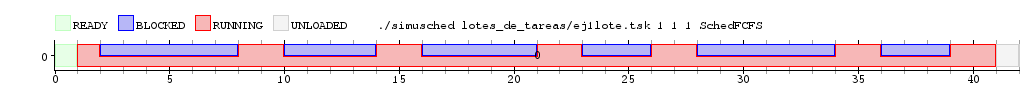
\includegraphics[width=500px]{imagenes/ej1.png}
		\caption{\small{\textbf{Gráfico generado con el lote.}}}
		\label{fig:grafico_ej1}
	\end{center}
\end{figure}
